\chapter{\sffamily Simple state transitions}

{\bfseries\sffamily Concept.} To define and develop an archetype simulation environment for simple state transitions. In our classification scheme, this archetype is defined by a trivial state partition graph topology and would make sense for simulations of sequential design problems, sports matches and other simple gameplay domains. We will also discuss the typical ways in which the state of the system may only partially be observed in realistic examples, and analyse how best to deal with each situation. For the mathematically-inclined, this chapter will define the mapping of our formalism to simple state transitions. For the programmers, the software which is designed and described in this chapter can be found in the public Git respository here: \href{https://github.com/worldsoop/worldsoop}{https://github.com/worldsoop/worldsoop}.


\section{\sffamily Defining the archetype}

The simple state transition archetype refers to simulation environments where there is no obvious computational benefit to partitioning the state into concurrently updating or acting on separate components. There may even be performance benefits from keeping state information all within the same common data structure in memory, but this can depend on the specific problem of study. 

In the interest of completeness with respect to the chapters which follow on from this one, we have illustrated the trivial state partition graph topology for this archetype in Fig.~\ref{fig:state-partition-graph-simple-state-transitions}.

In order to understand what sorts of data might be collected about this archetype in realistic scenarios, let's begin by considering the types of real-world problem domain which have leveraged simulation environments to train control algorithms in the literature. The subset of these which may best suit the simple state transition environment archetype are:
%%
\begin{itemize}
\item{Event-based simulations of sports matches, e.g., football~\cite{pulis2022reinforcement}, rugby~\cite{sawczuk2022markov}, tennis~\cite{ding2022deep}, etc., and other forms of game --- all of which typically define a relatively simple global match/gameplay context as their `state'.}
\item{Sequential design simulations to change the configuration or data collection strategies of, e.g., astronomical telescopes~\cite{jia2023observation,yatawatta2021deep}, biological experiments~\cite{treloar2022deep} and user interfaces~\cite{lomas2016interface}, which typically define a relatively simple and finite set of possible actions that can be taken.}
\end{itemize}
%%

\begin{figure}[h]
\centering
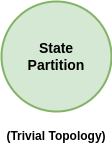
\includegraphics[width=2cm]{images/chapter-6-state-partition-graph.drawio.png}
\caption{State partition graph topology for simple state transition archetypes.}
\label{fig:state-partition-graph-simple-state-transitions}
\end{figure}

Based on the examples given above, what kinds of data may be available to infer the state and parameters of a simulation environment using this archetype? 

In the case of team sports matches, a team manager could have access to a large body of data which assesses the capabilities of their players before a game, but they must rely on more subjective or limited data to assess the performance of their team (and the opposition) in the middle of a match. The `state' of the whole system in this case can be not only the state of play, but also information about, e.g., fatigue or on-the-day performance of each player for both teams and sets of substitutes. 

\textcolor{red}{Talk about sequential design data here...}

In a general offline learning setting, realistic historical data collected about the state values for this archetype will typically provide an important mechanism for model determination. Users of this archetype in the real world also typically have access to independent datasets that can be used offline to better determine some parameters of the simulation environment which are not observed directly. In the online learning setting, one typically directly observes some portion of the state values, and may only indirectly observe the other state values, if at all.

\textcolor{red}{Within this topological archetype there will also be other categories to think are applicable:
\begin{itemize}
\item{Types of observation that can be made about the state.}
\item{Types of action that can be taken by an agent.}
\item{Types of agent? How frequently do these actions get taken? On what part of the state?}
\end{itemize}
}


\textcolor{red}{Types of actor:
\begin{itemize}
\item{sports team manager and other game player 1. substitute players 2. changes to tactics}
\item{public health authority and wildlife/national park control authority and livestock/crop farmer 1. spatially detect disease or damage 2. change state of a subset of the population}
\item{brain doctor and traffic light controller and city infrastructure maintainer 1. change the state of a subset of nodes in the network}
\item{supply/relief chain controller and hospital logistics manager and data pipeline controller 1. modify the relative flows between different pipeline stages}
\item{financial/betting/other market trader and market exchange mediator 1. interact with the market using an agent or collection of agents}
\end{itemize}}

\section{\sffamily Writing the code}

